\documentclass[tikz,border=4pt]{standalone}
\usepackage{amsmath,bm}
\usetikzlibrary{arrows.meta,calc,patterns}
\begin{document}
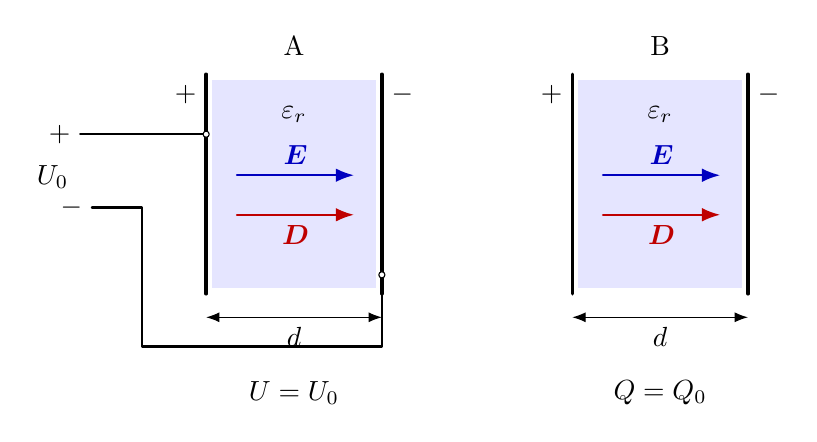
\begin{tikzpicture}[scale=0.93,>=Latex,line cap=round,line join=round]
  \tikzset{
    plate/.style={very thick},
    wire/.style={thick},
    field/.style={->,thick,blue!75!black},
    dfield/.style={->,thick,red!75!black}
  }

  \newcommand{\capdraw}[2]{
    \begin{scope}[shift={(#1,#2)}]
      \draw[plate] (0,0) -- (0,3.0);
      \draw[plate] (2.4,0) -- (2.4,3.0);
      \fill[blue!10] (0.08,0.08) rectangle (2.32,2.92);
      \node at (1.2,2.45) {$\varepsilon_r$};
      \node[left] at (0,2.72) {$+$};
      \node[right] at (2.4,2.72) {$-$};
      \draw[field] (0.42,1.62) -- (2.02,1.62) node[midway,above] {$\bm E$};
      \draw[dfield] (0.42,1.08) -- (2.02,1.08) node[midway,below] {$\bm D$};
      \draw[<->] (0,-0.32) -- (2.4,-0.32) node[midway,below] {$d$};
    \end{scope}
  }

  % A: the source is still connected, so the voltage is fixed.
  \capdraw{0}{0}
  \node at (1.2,-1.35) {$U=U_0$};
  \node at (1.2,3.38) {$\mathrm{A}$};
  \draw[wire] (-1.72,2.18) -- (-1.02,2.18);
  \draw[wire] (-1.56,1.18) -- (-1.18,1.18);
  \node[left] at (-1.72,2.18) {$+$};
  \node[left] at (-1.56,1.18) {$-$};
  \node[left] at (-1.75,1.60) {$U_0$};
  \draw[wire] (-1.02,2.18) -- (0,2.18);
  \draw[wire] (-1.18,1.18) -- (-0.88,1.18) -- (-0.88,-0.72) -- (2.4,-0.72) -- (2.4,0.26);
  \draw[fill=white,draw=black] (0,2.18) circle (1.2pt);
  \draw[fill=white,draw=black] (2.4,0.26) circle (1.2pt);

  % B: after charging, the capacitor is isolated; only the free charge stays fixed.
  \capdraw{5.0}{0}
  \node at (6.2,-1.35) {$Q=Q_0$};
  \node at (6.2,3.38) {$\mathrm{B}$};
\end{tikzpicture}
\end{document}
